
\chapter{相关工作}

\section{相关的理论研究工作}

软件性能测试一直是软件工程里面一个比较重要的话题,与之相关的理论研究也比较多,如Skoll\cite{schmidt2001leveraging}和.........是其中比较优秀的研究。

\subsection{利用社区提高开源软件质量}

\subsection{自动性能分析}

\section{相关工程项目}

Linux内核作为一个庞大和复杂的系统软件,很早之前就已经引起了很多公司或团体的注意,并以之为测试目标,开发了比较实用,比较方便的进行Linux性能测试的工程项目,比如LKP\cite{chen2007keeping},TKO\cite{bligh2006fully}和MMTests就是其中两个比较优秀的工程项目。

\subsection{Linux Kernel Performance}

Linux Kernel Performance(简称LKP),是Intel公司的开源技术中心于2005年开始的一个用于进行Linux内核性能测试的一个测试框架。

由于Linux内核的快速发展,Intel开源技术中心的一部分工程师开发了一套对Linux内核性能进行测试的框架,这套框架的具体架构如图\ref{fig:old_lkp_arch}

\begin{figure}[H]
\centering
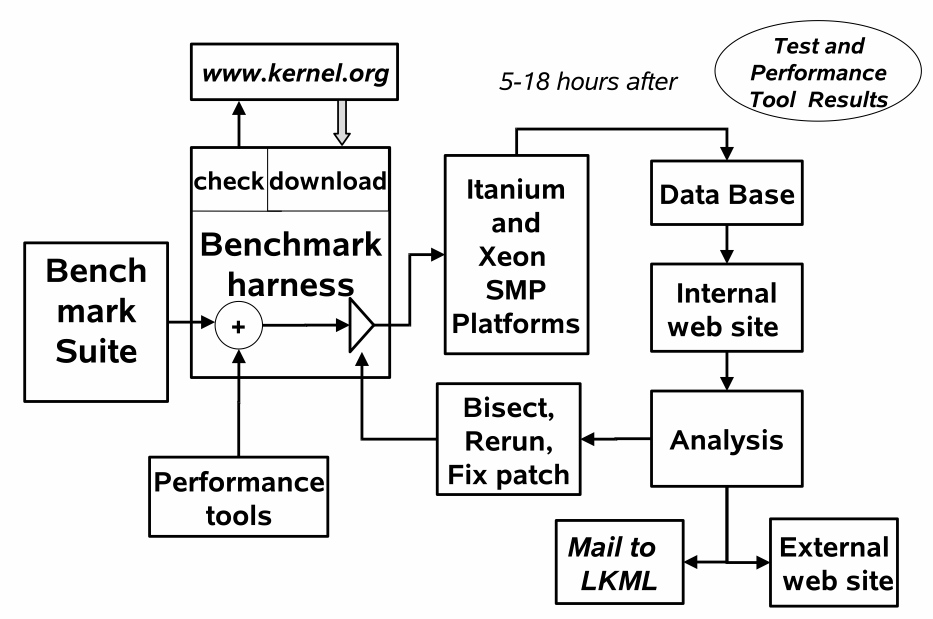
\includegraphics[width=10cm]{old_lkp_arch}
\caption{LKP测试框架架构}
\label{fig:old_lkp_arch}
\end{figure}

在这套框架中,主要的测试分为5个阶段,分别是:
\begin{enumerate}
\item 下载代码并编译。首先从linux.org网站上面下载各个版本的内核源代码,并进行编译,一般都只是对具有tag的版本(包括RC版本和最终发行版)进行编译。
\item 运行测试。使用上一个阶段中编译好的内核来启动一台物理机器,并在这一台物理机器中运行各种各样的测试例程,如Kbuild,Reaim7,Netperf,Tbench等比较经典和常用的测试例程。同时,在测试例程运行的过程中,还会启动vmstat,iostat,sar,ps等工具来进行测试数据的采样和收集,采集到的数据都将被保存在数据库中,方便在后来进行查询。
\item 结果分析。根据在上一个阶段中收集到的测试数据,作出相关的数据统计分析,同时结合每一个测试例程的运行结果来给每一次的测试进行评分。在评分的过程中,给予每一个不同的测试例程相应的权重值,然后根据权重值计算出本次测试的得分,然后通过得分来判定性能的变化情况。
\item 问题查找。如果在进行结果分析的时候发现了性能回退的情况,那么就会在Linux内核的代码树中使用git-bisect来进行问题的查找,定位出问题发生的位置和原因,然后将问题的定位和分析结果通过邮件的形式发送给Linux内核的邮件列表中。
\item 结果呈现。将测试的结果通过不同的形式展示出来,在LKP中提供一个web界面进行测试数据的浏览,数据会以表格或者图表的形式进行展示,方便开发者们查看数据变化的趋势。
\end{enumerate}

在任何的测试系统中,测试时的波动都是需要考虑的内容,在LKP中同样也不例外。

LKP中对测试时发生的波动的处理可以说是比较简单,但是同样也是比较有效的,其中采用的具体措施有以下几个:
\begin{enumerate}
\item 每次都在一个已知的系统状态上开始测试
\item 在进行正式的测试之前,会使用一些简单的测试例程来使得系统到达一个比较稳定的状态
\item 通过进行长时间的测试以及多次运行测试例程后取平均值来得到最终的测试结果
\end{enumerate}

然而,这样的措施虽然能够在一定的程度上降低测试波动造成的影响,并能够检测到一些比较严重的性能回退问题,但是一些较小的性能回退仍然有可能会混淆在测试的波动中。


\subsection{TKO}
TKO指的是一个运行在http://test.kernel.org网站上面的一个Linux内核测试和测试结果发布系统。

在TKO中,提高一个软件的质量被认为是下面各个方面综合的结果:
\begin{itemize}
\item 使用优秀的程序员编写优秀代码
\item 静态代码分析
\item 常规的严格代码审阅机制
\item 新特性的功能测试
\item 回退测试
\item 性能测试
\item 压力测试
\end{itemize}
于是,根据这样的思想指导,TKO设计的总体框架如图\ref{fig:tko_arch}所示。

\begin{figure}[H]
\centering
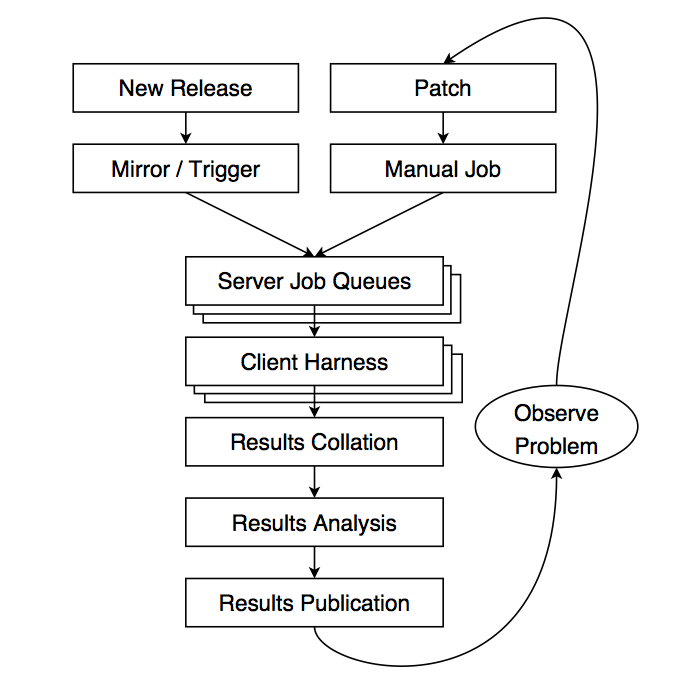
\includegraphics[width=10cm]{tko_arch}
\caption{TKO框架架构}
\label{fig:tko_arch}
\end{figure}

TKO主要有下面几个功能模块:
\begin{itemize}
\item[\heiti{镜像触发引擎:}] 当kernel.org上发布了新的内核版本的时候,会触发该引擎,从kernel.org上面下载最新的内核镜像。
\item[\heiti{服务器工作队列:}] 对于每一个新的内核都会有一系列需要任务需要运行,这些任务都将在该队列中进行调度。
\item[\heiti{客户端管理:}] 该模块运行在进行测试的客户端机器上,当有新的内核需要运行的时候,这个模块将会管理整个测试的运行流程,负责完成客户端机器上的测试例程运行管理。
\item[\heiti{结果收集:}] 负责在测试例程完成之后,异步地从客户端机器上相应的任务中收集测试信息,并保存在数据库中以备后用。
\item[\heiti{结果分析:}] 根据收集到的所有信息进行分析,在这个环节中,需要进行性能分析,所以需要将历史的性能数据保存下来,这样可以画出比较完整的性能变化曲线。
\item[\heiti{结果发布:}] 在完成了结果分析之后,将分析得到的结果发布到TKO的网站上面,同时还需要在测试出现意外或者错误的时候通知开发者社区。
\item[\heiti{问题监测:}] 这个模块会对测试和分析的结果进行监测,一旦监测到问题,同样会通报给开发者社区,之后可以手动地向任务队列中添加任务对出现的问题进行确认。
\end{itemize}

根据相应论文的描述,TKO系统只是一个原型系统,只能完成的简单的测试和结果发布,还不能进行比较复杂的测试数据分析和问题的定位,尽管如此,TKO已经提出了一套比较完整的内核测试流程,给后人设计和开发类似的系统提供了有价值的经验。


\subsection{MMTests}

MMTests是一个可配置性极强的测试套件,这个测试套件是为Linux内核的内存管理(MM)子系统的开发者开发的,在这个测试套件中,包含并整合了大量的测试例程,其中有比较著名的Linux Test Project(LTP),xfstests以及Phoronix Test。

相比于LKP,MMTests具有以下优势:
\begin{itemize}
\item 具有更强的可配制性。在MMTests中,只需要编写简单的配置文件,就可以比较轻松地往MMTests中添加新的测试例程,同样,可以通过简单地修改配置文件来达到进行不同测试参数地修改
\item 获得更全面的测试数据。MMTests中包含有更多的系统监视器(monitor),拥有更多的系统监视器意味着能够得到更加全面,更加完整的测试数据,从而在寻找性能回退问题的时候具有更高的敏感性。
\end{itemize}

但是,归根到底,MMTests仅仅是一个测试套件,而并不是一个完整的测试框架,不能完整地进行指定内核的所有测试流程,这是因为MMTests并不具备内核编译、数据分析、问题定位等对于完整测试框架来说颇为重要的功能。




